\chapter{New Material Design GUI}
\label{gui}

In this short chapter i'll show the main improvements to the GUI.
Mainly, I used all available elements into the support library and I replaced the Holo Theme with ``Theme.AppCompat.Light.NoActionBar" to mimic the Material Theme. Also, when necessary, I used the Compat element, like CompatButton and so on to show the same element in different Android's versions. When possibile I replaced unofficial libraries or old component with the new Google Design support library, for example to crete tab layouts. 

\begin{figure}[thpb]
\centering
\begin{minipage}[b]{0.4\textwidth}
	\centering
	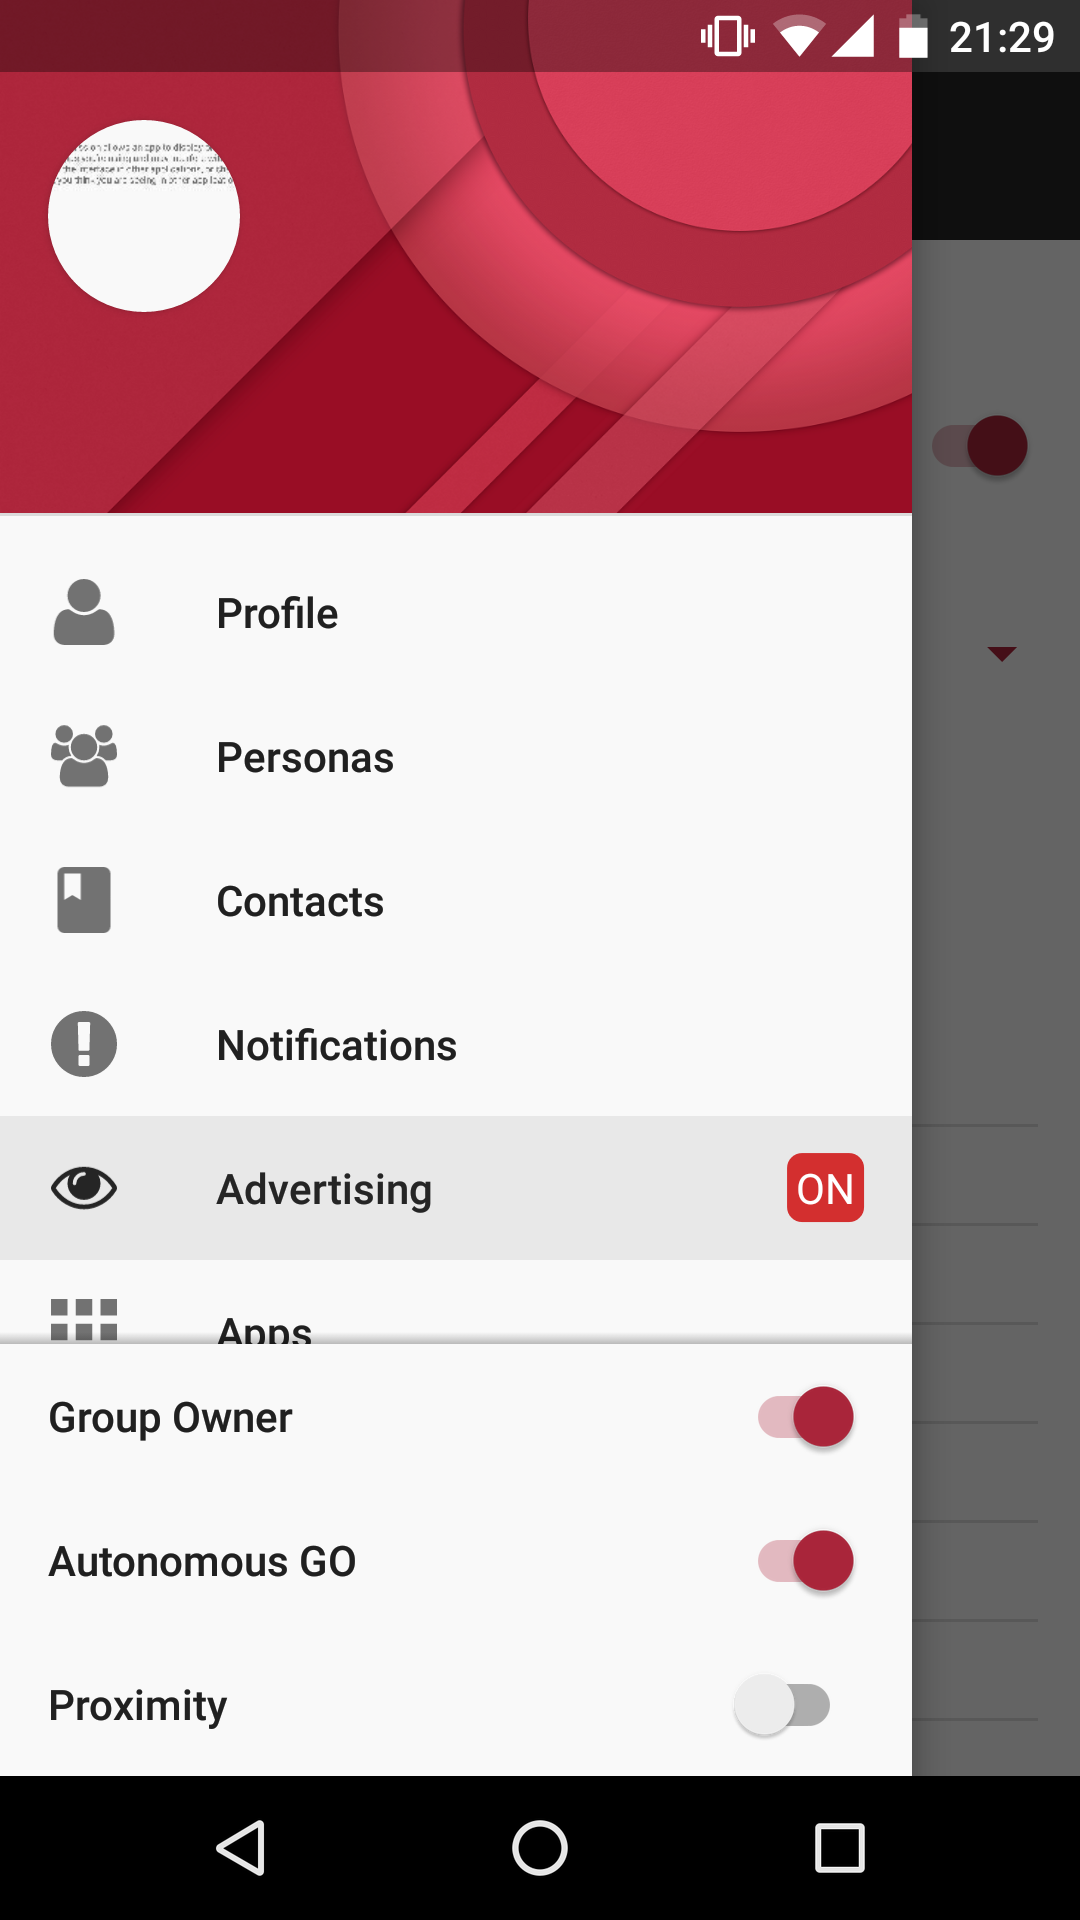
\includegraphics[scale=0.1]{./images/chap3/drawer.png}
	\caption{Drawer}
	\label{fig:drawer}
\end{minipage}
\hfill
\begin{minipage}[b]{0.4\textwidth}
	\centering
	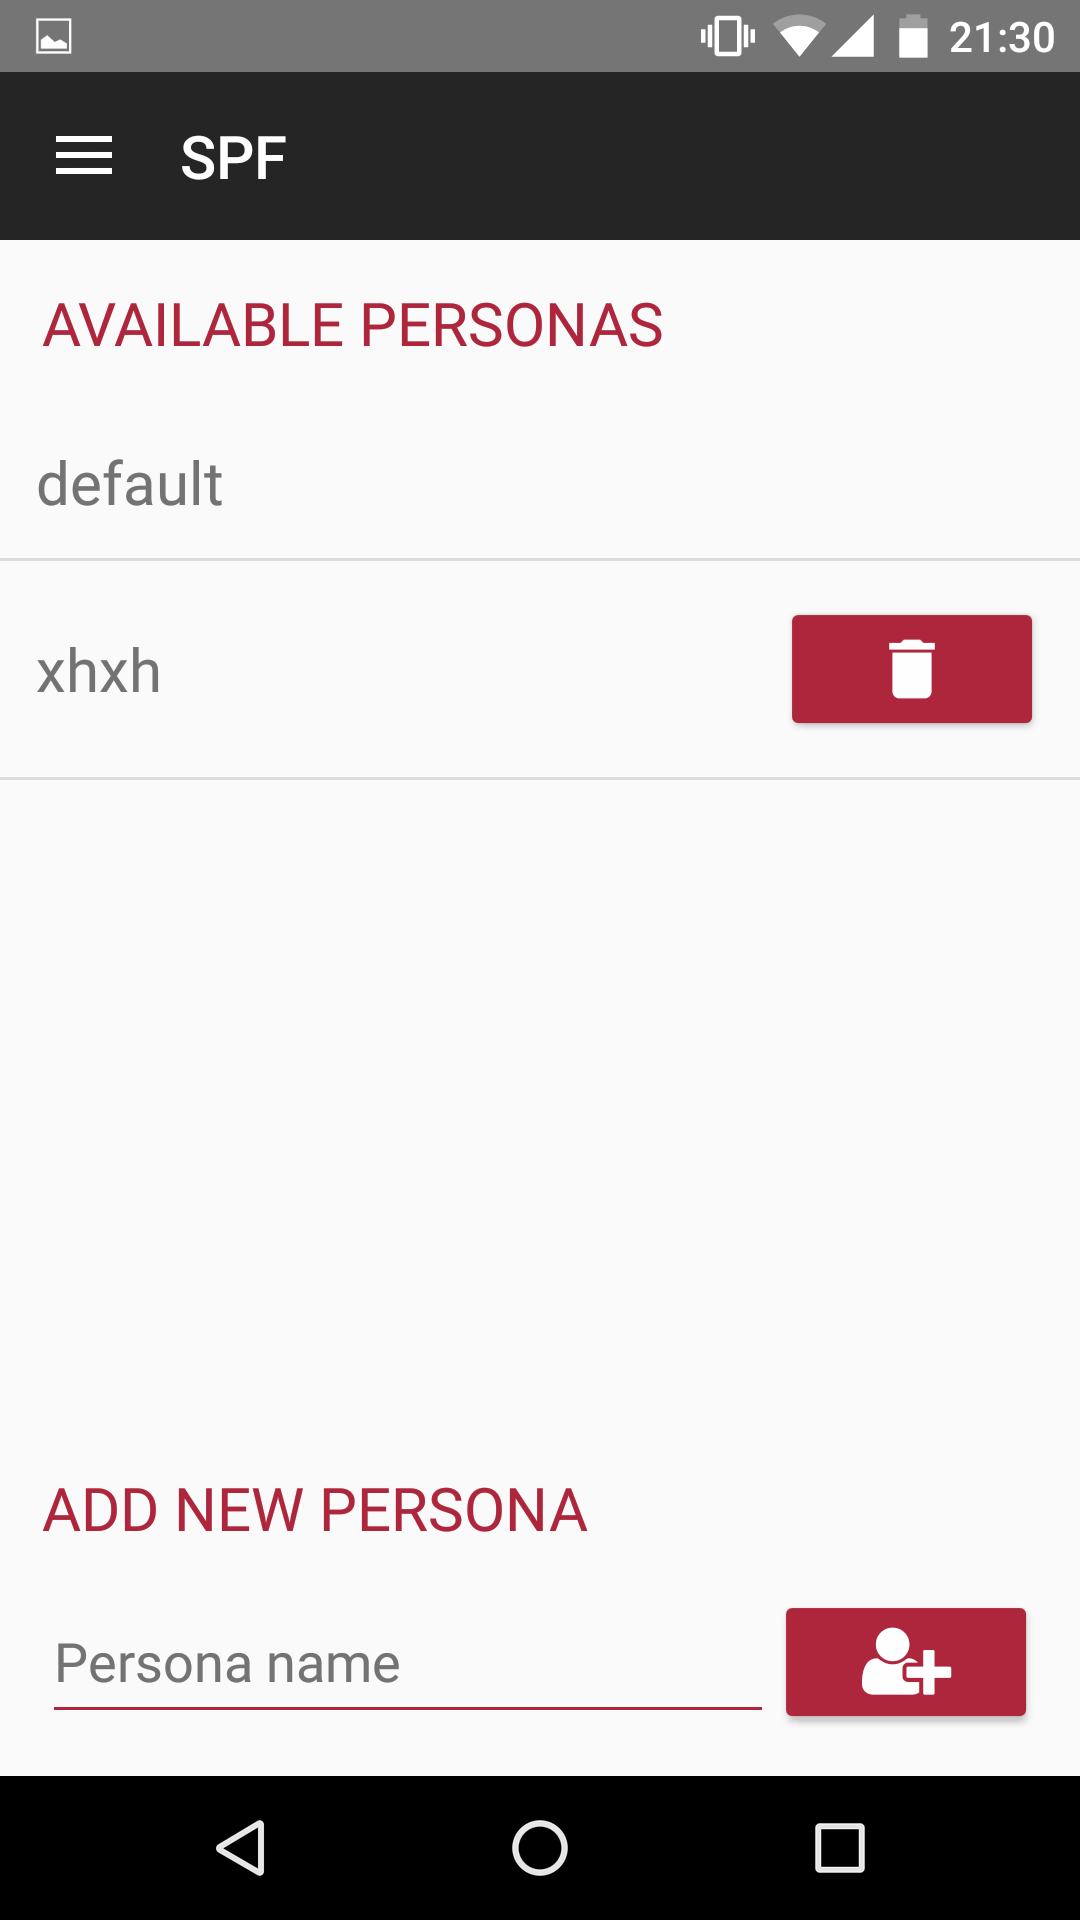
\includegraphics[scale=0.1]{./images/chap3/bottom_iconics.png}
	\caption{Buttons with Iconics}
	\label{fig:buttom-iconics}
\end{minipage}	
\end{figure}	

I applied all this updates to all SPF's apps. Also, I implemented the Material Drawer using a custom unofficial library available on GitHub, created by Mike Penz. The idea was to build a cool Material Drawer very quickly without to implement manually some annoying features. The result is in Figure \ref{fig:drawer}. In addition, I used Iconics library to add vector icons to buttons, toolbar and to the drawer's items, as in Figure \ref{fig:buttom-iconics}.

\begin{figure}[thpb]
\centering
\begin{minipage}[b]{0.4\textwidth}
	\centering
	
\includegraphics[width=\textwidth]{./images/chap3/header.png}
	\caption{Header}
	\label{fig:header}
\end{minipage}
\hfill
\begin{minipage}[b]{0.4\textwidth}
	\centering
	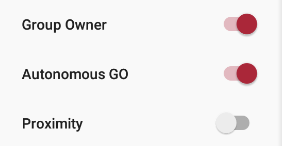
\includegraphics[width=\textwidth]{./images/chap3/switches.png}
	\caption{Drawer's switches}
	\label{fig:switches}
\end{minipage}	
\end{figure}



As you can see, i added a Header with an image and the profile photo (Figure \ref{fig:header}) and a Sticky Footer into the drawer, with switches (Figure \ref{fig:switches}). Also, I added two new items: Group Infos and About. The first one selects a fragment with the available services and the connected devices. This is not necessary to users, but it very useful during development to understand if a device is still connected or if there are problems related to Wi-Fi Direct. The second one is a simple about page of SPF, created with a library that compose this Activity scanning the libraries and dependencies used inside this application, automatically.

\begin{figure}[thpb]
	\centering
	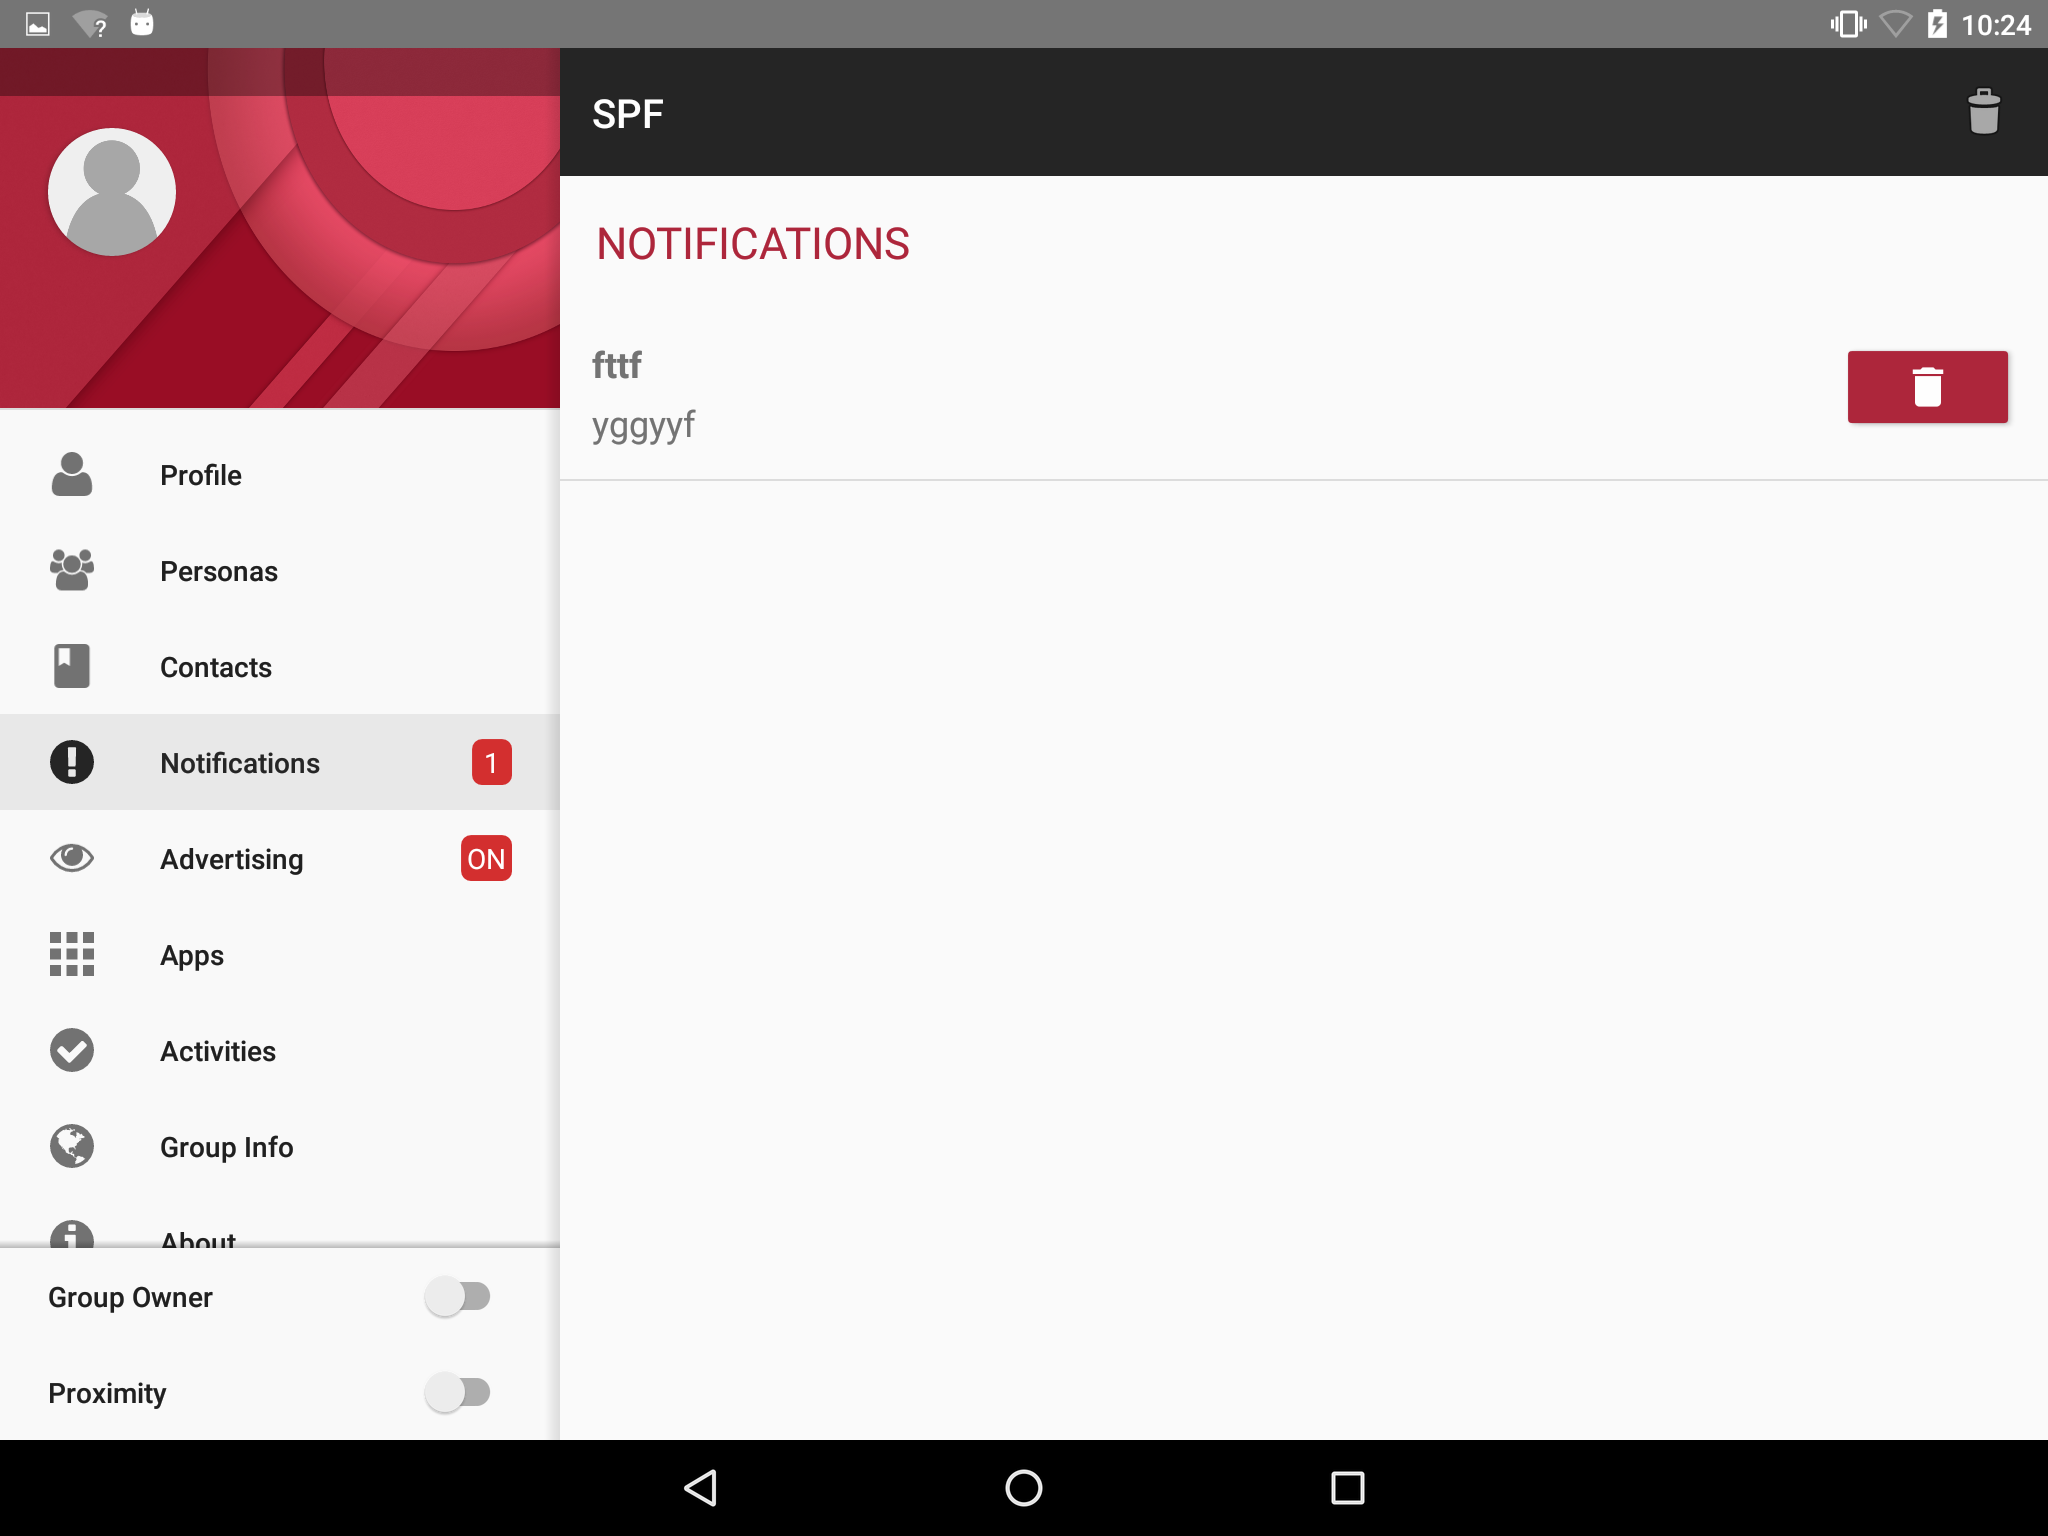
\includegraphics[scale=0.3]{./images/chap3/tablet1.png}
	\caption{Multi-pane layout}
	\label{fig:tablet1}
\end{figure}	


After this quick explanation i want to explain one of this features, i.e. the Material Drawer, in particular how to reuse the same Drawer for smartphone and Tablets to create a Multi-pane layout, as in Figure \ref{fig:tablet1}.

In Listing \ref{lst:multipane} there is a shorter version of the code that I used to create the drawer. All the method's invocations are chained, because every method returns always the same object, DrawerBuilder.


\begin{lstlisting}[caption={DrawerBuilder creations},label=lst:drawerbuilder, language=Java]
drawerBuilder = new DrawerBuilder()
  .withActivity(this)
  .withAccountHeader(headerResult)
  .withHasStableIds(true)
  .withToolbar(toolbar)
  .addDrawerItems(
    new PrimaryDrawerItem().withName(mSectionNames[0])
      .withIdentifier(0).withIcon(FontAwesome.Icon.faw_user),
    	(...)
  )
  .withOnDrawerItemClickListener(drawerItemClickListener)
  .withSavedInstance(savedInstanceState);
\end{lstlisting}


And finally, in Listing \ref{lst:multipane} I added the code to reuse the MaterialDrawer to create a Multipane layout. The trick is to the view obtained from the drawer to the viewGroup related to the layout's element, a simple FrameLayout that I called \textsf{nav\_tablet}. Obviously you need two layouts, one for smartphones and one for tablet. In the first case you must use a DrawerLayout, in the second one you could simply use a FrameLayout.


\begin{lstlisting}[caption={Reuse Drawer for Multi-pane layout},label=lst:multipane, language=Java]
if (tabletSize) {
  //if tablet create a multipane layout
  drawer = drawerBuilder.buildView();
  ((ViewGroup) findViewById(R.id.nav_tablet))
    .addView(drawer.getSlider());
} else {
  //on smartphones i want to show the hamburger icon
  if (getSupportActionBar() != null) {
    getSupportActionBar().setDisplayHomeAsUpEnabled(false);
  }
  drawerBuilder.withActionBarDrawerToggle(true);
  drawerBuilder.withActionBarDrawerToggleAnimated(true);
  drawer = drawerBuilder.build();
  drawer.getActionBarDrawerToggle()
    .setDrawerIndicatorEnabled(true);
}
\end{lstlisting}


